
\section{Abstract}
With the increasing demands of higher education, small but necessary routine tasks can become time-consuming and burdensome for busy college students. To address this issue, we propose a design for an online marketplace that enables college students to outsource their routine tasks to other students. This marketplace aims to facilitate the efficient offloading of small tasks, creating value for both the task requester and performer. Tascii's design is catered towards college students with a minimal design that draws inspiration from social media platforms. Leveraging the existing trust that is built into a college community, the design is flexible and unobtrusive where most other peer-to-peer platforms are prohibitive. Our analysis of competitors helped to identify critical features for our platform, and through an iterative design process, we began to hone our application's user experience. Usability studies and heuristic evaluation helped to inform our high-fidelity prototype as we addressed issues with clarity and navigation. As we develop a peer-to-peer market specifically for a college campus, our study can inform the design of future systems that aim to encourage cooperative and community-driven behaviors among users.

\section{Introduction}

As the demands of higher education continue to increase, students often find themselves overwhelmed with small yet necessary routine tasks that take up valuable time. To address this issue, our team proposes a design for an online marketplace where college students can outsource tasks to other students for a set price. Lampinen and Brown, in there research on markets and HCI, note that "markets are essentially social systems and when we design new collaborative platforms, we inherently adopt some assumptions about a social system – or create new social systems."\footnote{Market Design for HCI: Successes and Failures of Peer-to-Peer Exchange Platforms. https://dl.acm.org/doi/pdf/10.1145/3025453.3025515} With this in mind, our platform is built  around the needs of a specific social system. We aimed to create a platform that not only facilitates transactions but also encourages cooperative and community-driven behaviors among users. Through a combination of initial observations, case studies, and surveys, we sought to explore the problems faced by busy students and the potential impact of our solution.

We collected initial observations as several of our roommates texted in a group chats to look for help with tasks around campus. For example, one student said they were willing to Venmo \$10 to whoever could move their car, but unfortunately everyone in the chat was busy. To follow up on these initial observations, we constructed a need-finding survey to gauge interest in the concept on campus. By placing posters with QR codes and actively distributing the survey, we obtained valuable insights that helped shape our product development process. The data collected allowed us to create personas and scenarios, illustrating how users would engage with our system. The survey yielded encouraging results, with significant interest from students across a range of different use cases. The survey received 36 responses, revealing that 53.6\% of respondents would pay someone to move their car, and 60.7\% would pay for something from Thorne Dining Hall's SuperSnacks. The survey also revealed unexpected demand for package pick-up services. Additionally, respondents indicated that they would be interested in being paid to do these tasks. Figures 11 and 12 in the appendix illustrate the presence of supply and demand and a market clearing price. These findings suggest that there is considerable interest in the platform, and they indicate a diverse range of needs to consider in its implementation. With this feedback, we aimed to integrate flexibility into the core of our concept's implementation.

In a tight-knit community such as Bowdoin's campus, students are already collaborative and willing to help, yet they lack the resources to connect with other students. Furthermore, need-finding results show that there is a willingness to participate such transactions. Tascii aims to provide a convenient solution for students to offload small tasks in a way that generates surplus for both parties involved in the transaction.

We examined a series of competitors to identify the components that makes their platforms successful, and building on these findings, we developed a series of prototypes to incorporate feedback from users. With our unique peer-to-peer marketplace, Tascii contributes by exploring a new market context and interface design which promotes unprecedented flexibility. To evaluate the effectiveness of our application, we designed a study to compare aesthetics and user efficiency with a competing application.


\section{Related Work}

\subsection{Competitive Analysis}

The gig economy (market for one time free lance jobs) has seen rapid growth in recent years as multiple online marketplaces have emerged. Peer-to-peer platforms such as Uber, DoorDash, Craigslist, Fiverr, and Taskrabbit all host their own unique marketplace to target different problems. Each employs a unique market structure as a part of their solution, and it is important to first recognize the problems that any marketplace must address. Lampinen and Brown have proposed an HCI framework for evaluating market design.\footnote{Market Design for HCI: Successes and Failures of Peer-to-Peer Exchange Platforms. https://dl.acm.org/doi/pdf/10.1145/3025453.3025515} They identified thickness, congestion, safety, stability, and repugnance as key concepts to characterize a market. Thickness refers to the number of participants the market attracts, and congestion relates to the ease with which participants can navigate a thick market. Market safety ensures that participants are served reliable information and they face little risks. In a stable market, people can not find an outcome that is mutually more beneficial. Lastly, repugnance refers to the moral connotations associated with the market.\footnote{Ibid} With these concepts established, they can be applied to highlight similarities and differences between each competitor. 
 
Uber represents the epitome of disruption and rapid growth in the new sharing economy. In pairing personal service and technology, the platform makes use of assets which traditionally had unrealized value. Uber’s design is centered around seamless transactions and quick matchmaking between drivers and consumers. As opposed to traditional marketplaces, the producers are forced to meet consumers where they are, adding to convenience.\footnote{Smith, J. Walker. “The Uber-All Economy of the Future.” The Independent Review 20, no. 3 (2016): 383–90. http://www.jstor.org/stable/24562159.} However, Uber has faced controversy with respect to their dynamic pricing scheme. Uber changes its prices based on the supply and demand at any given time, and a study from the Australian National University found that  “although a dynamic pricing strategy improves efficiency, it is incredibly annoying. In the passengers’ opinion, the most annoying part is the price increase when they need a car urgently.” There is a tradeoff between flexible pricing and consistency, which each competitor in this analysis tackles differently. Uber handles congestion well as matches are made seamlessly, but in more rural locations there have been issues with thickness. Since launching they have responded to safety concerns by posting yearly safety reports and releasing new in-app features for emergency situations.\footnote{Uber. "Safety." https://www.uber.com/us/en/ride/safety/?uclick_id=58abd988-91d0-4969-97d0-423a3dd436d2.}

DoorDash partners with restaurants to gain their own competitive advantage in food delivery. They rely on these partnerships to determine prices for their online menus. Here, the price of a delivery is usually the cost of the food plus a delivery fee and a tip. Similar to Uber’s model, customers place an order on their app and they are automatically matched with the most convenient delivery person nearby. One inconvenience is that the signup process for both Uber and DoorDash are both heavily involved. Applicants need to send insurance and vehicle information along with consenting to a background check. While somewhat frustrating for users, such measures serve to boost credibility and the reputation of the service. 

Taskrabbit is another platform that matches customers with nearby “taskers” who are available to help with household chores. Taskers are required to submit business certifications, consent to a background check, and pay a \$25 signup fee. Users select a task category and are instantly matched with someone who has availability at that time. However, Taskrabbit is only available in major cities, and it caters to workers who are able to specify their hours ahead of time. 

In Good Jobs, Bad Jobs, in the Gig Economy, Kalleberg and Dunn investigate the different frameworks platforms employ to find matches for workers online. In their work, they construct a matrix to delineate between platforms where workers are paid well and where they have control over prices. From this perspective, Uber and DoorDash are both characterized by high wages and low control. In settings with short term, unskilled work, the platform must seize more control in order to act as a reputable source.\footnote{Kalleberg, Arne L., and Michael Dunn. “Good Jobs, Bad Jobs in the Gig Economy.” Perspectives on Work 20 (2016): 10–75. http://www.jstor.org/stable/26621129.} In contrast, platforms like Fiverr allow workers to determine their own price or hourly rate as the work is more subjective and skill-based. On Fiverr, customers pick from a wide range of freelancers and work iteratively to create a final product. Trust is a critical factor in all of these platforms, and each company adds features to address this to improve market safety.\footnote{An economic analysis of the Sharing Economy: A Case Study in Uber for taxis. (n.d.). https://openresearch-repository.anu.edu.au/bitstream/1885/216366/1/8180\%20Uber.pdf } Uber has the ability to rate other users, and most others allow you to inspect profiles and reviews for past work. With short term projects, mechanics for building reputation help ensure that suppliers provide a good experience to consumers. Fiverr, with its focus on artistic work, offers the most support in this regard as artists can post previous work and reviews.

On the other end of the spectrum, Craigslist postings are not accompanied by any reviews, and sellers are often anonymous. On Craigslist, users contact the seller and finalize the details of the transaction separately. Craigslist offers a wide variety of postings with a simplistic interface, but it is difficult to navigate. Creating a post is slow and costs \$25 per listed category. Additionally, it is difficult to verify the information in each post, resulting in an issue of market safety. The NYU Tandon School of Engineering recently published the first systematic study of Craigslist scams involved analyzing more than 2 million listings on Craigslist over a period of five months. The study found about 29,000 fraudulent listings in 20 major American cities. However, only 47 percent of these listings were flagged as "suspicious" by Craigslist.\footnote{Park, Haewoon. "Towards an Understanding of the Effects of Social Media on Political Participation." ACM CCS '16: Proceedings of the 2016 ACM Conference on Computer and Communications Security, ACM, New York, NY, USA, 2016, pp. 1065-1080.} Such issues along with the \$25 fee for each post discourage students from using these platforms. Our proposed application addresses this gap by providing a marketplace that is internal to Bowdoin students. Our application aims to create a social system that fosters collaboration and community-driven behaviors among Bowdoin students.

\begin{figure}[ht]
        \centering
        \caption{Competitive Analysis}
        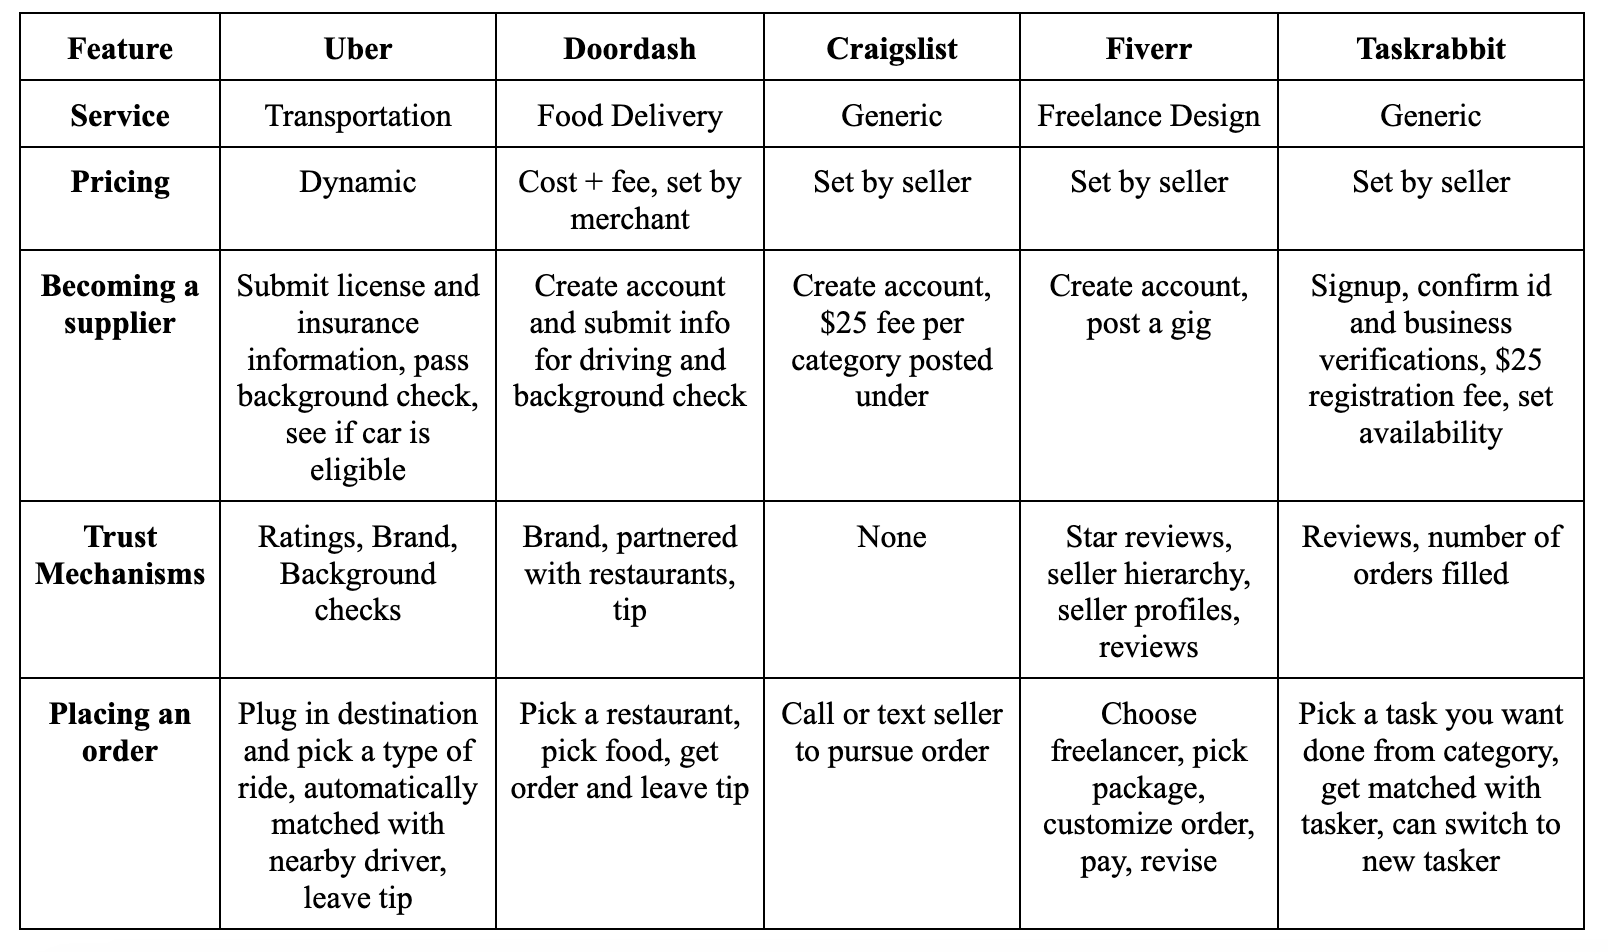
\includegraphics[width=1\textwidth]{images/competitors.png}
        
        \label{fig:bird1}
    \end{figure}


\subsection{Contribution}

Tascii is distinct from these competitors in a couple of key areas. First, our target demographic is far more specific than these other platforms. This would allow Tascii to leverage the trust that is already built into college communities. Reciprocity on online services is largely determined by community norms and anonymity.\footnote{Why do you return the favor in online knowledge communities? A study of the motivations of reciprocity. https://www.sciencedirect.com/science/article/pii/S0747563216303314} Having a preexisting community would help to boost engagement while providing support for users who are getting started with the service.\footnote{Learning to Airbnb by Engaging in Online Communities of Practice. https://dl.acm.org/doi/pdf/10.1145/3359330} Meanwhile, anonymity has been shown to increase free-riding, so we are looking to add more social features in the future. Working within a college community has the added benefit of speeding up the sign-up process, and we hope to integrate Bowdoin’s secure Okta sign-in. Most other services require background checks and credit card information, making the sign-up process a significant barrier to entry. Despite these contributions towards trust and market safety, there are still some issues with the current state of Tascii. For example, as of right now there is no way to report users or malicious posts. By adding this feature along with public profiles, the added accountability should help to increase the safety of the platform. Just as Uber profits from the unrealized value of pre-existing assets, Tascii is positioned to capitalize on common traffic among students on the same campus. 

Tascii also offers a unique interface for transacting with peers. Craigslist is perhaps functionally the most similar to Tascii, but its interface is outdated and difficult to navigate. Where Craigslist posts are more formal and take longer to make, Tascii is closer to texting friends to ask for a favor. Most competing marketplaces are outdated and not geared towards college students. Even Facebook's internal researchers predicted that their own marketplace would lose popularity among younger users.\footnote{ Roose, Kevin. "Facebook is Weaker Than We Knew." The New York Times, 4 Oct. 2021, https://www.nytimes.com/2021/10/04/technology/facebook-files.html.} With the target demographic of college students, our interface takes inspiration from social media more than E-commerce sites. The posting process is fast and offers unparalleled flexibility. As opposed to services like Uber and DoorDash, students have both the ability to set their own price and get paid well. 


\section{Approach}

The Tascii interface has been designed to cater to the specific needs of college students, offering a range of unique features that set it apart from other platforms. One notable feature is the ability to post tasks with references to custom locations on campus (see fig 2). Users are free to use natural language and the nicknames they would use in any message to a friend. This allows users to communicate their needs effectively while promoting a more casual tone that mirrors real world exchanges. Similarly, the title field allows users to put in emojis to make the message more fun and engaging. We wanted to streamline the posting process as much as possible, so the form only includes the essential information for a post. In our original form there were redundant fields that we were able to eliminate with default values. The first version of the form also made inputting dates extremely difficult. To help with this problem, the form includes a built-in calendar widget which is much more intuitive. Additionally, we changed the time estimate to a drop-down form with a few basic options to increase efficiency.

\begin{figure}[ht]
        \centering
        \caption{Making a Post}
        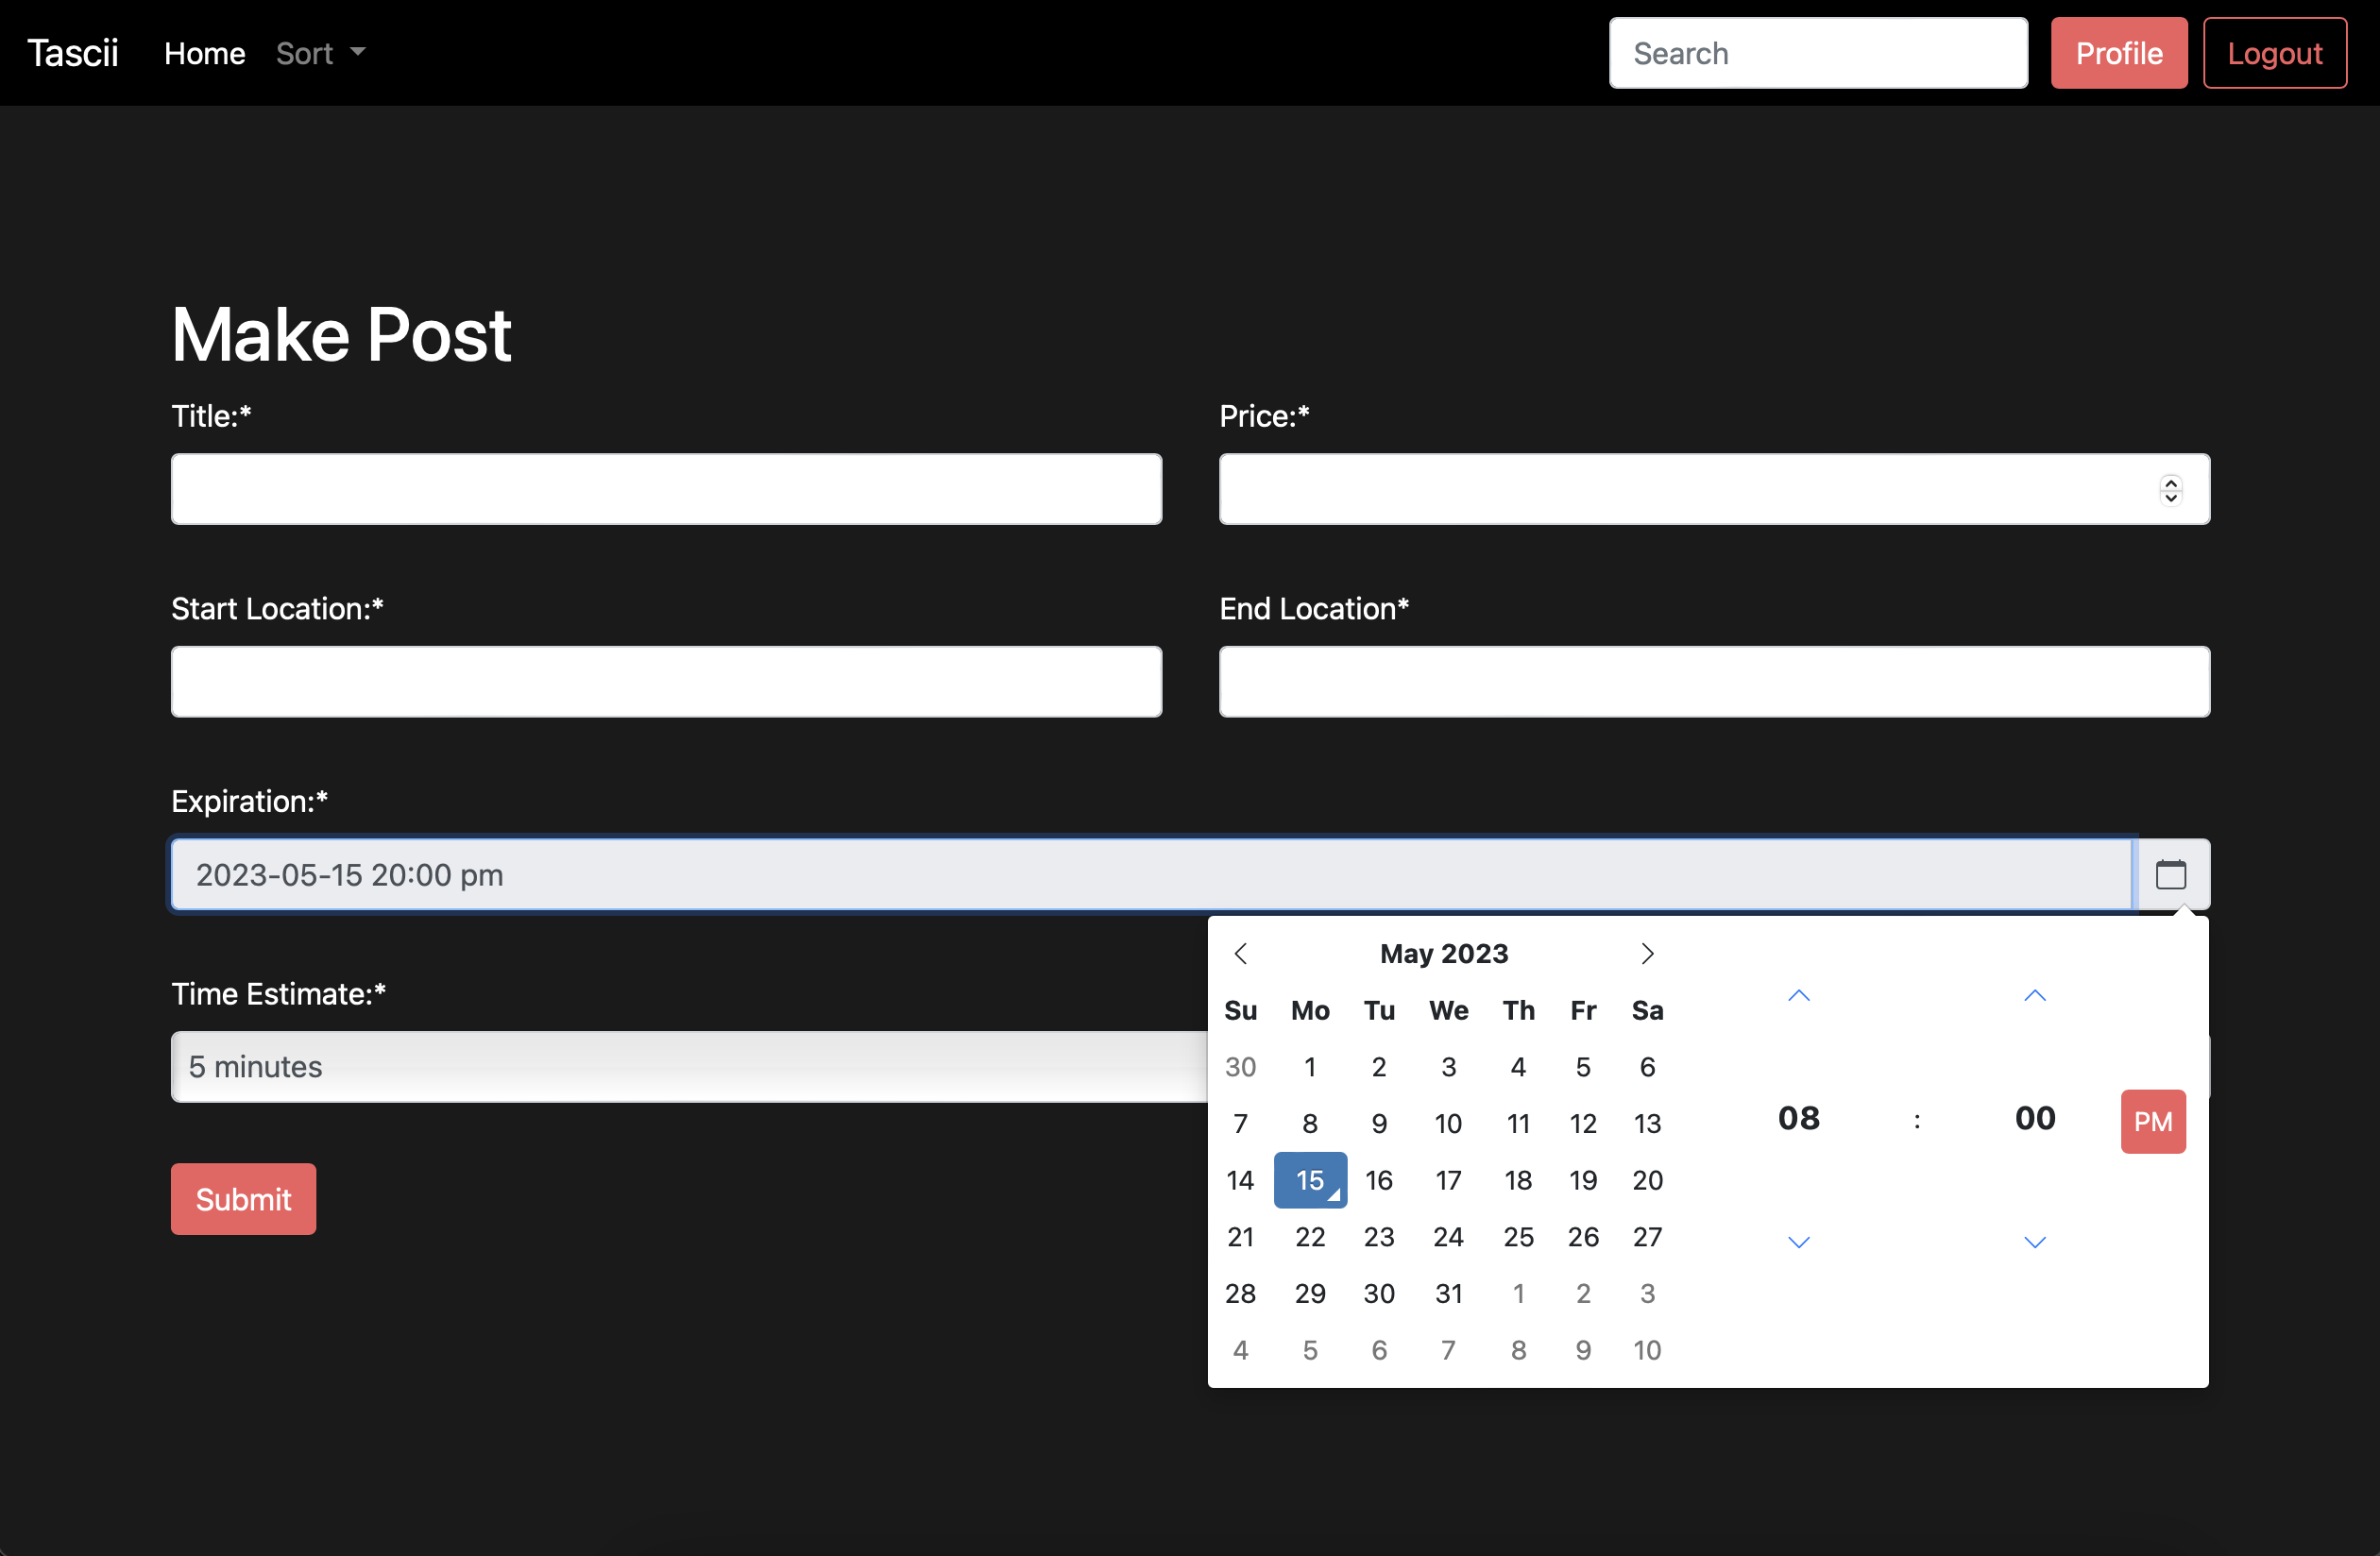
\includegraphics[width=1\textwidth]{images/Make Post.png}
        
        \label{fig:bird1}
    \end{figure}

The form for editing a post mirrors the form for making a post in the first place, but all of the fields are automatically filled to reflect the current state of the post. It also allows users to take down a post, so that they are able to recover from a mistake easily. While this page isn't very flashy, it is essential for error recovery and user control. In terms of error prevention, we had the accept button on the home page lead to a secondary page with more information that would serve as a sort of confirmation.

In the home page, the posting button itself has been intentionally designed as the largest components across all pages, considering Fitt's Law of Human Movement (see fig. 3). The law states that the time required to point to a target depends on the distance to the target midpoint and the width of the target. In line with this principle, we have ensured that the button is wide enough to facilitate easy and accurate selection. The size of this component also establishes a clear hierarchy that guides users towards this main action at the bottom of the page.

\begin{figure}[ht]
        \centering
        \caption{Home Page (with 'Make Post' button)}
        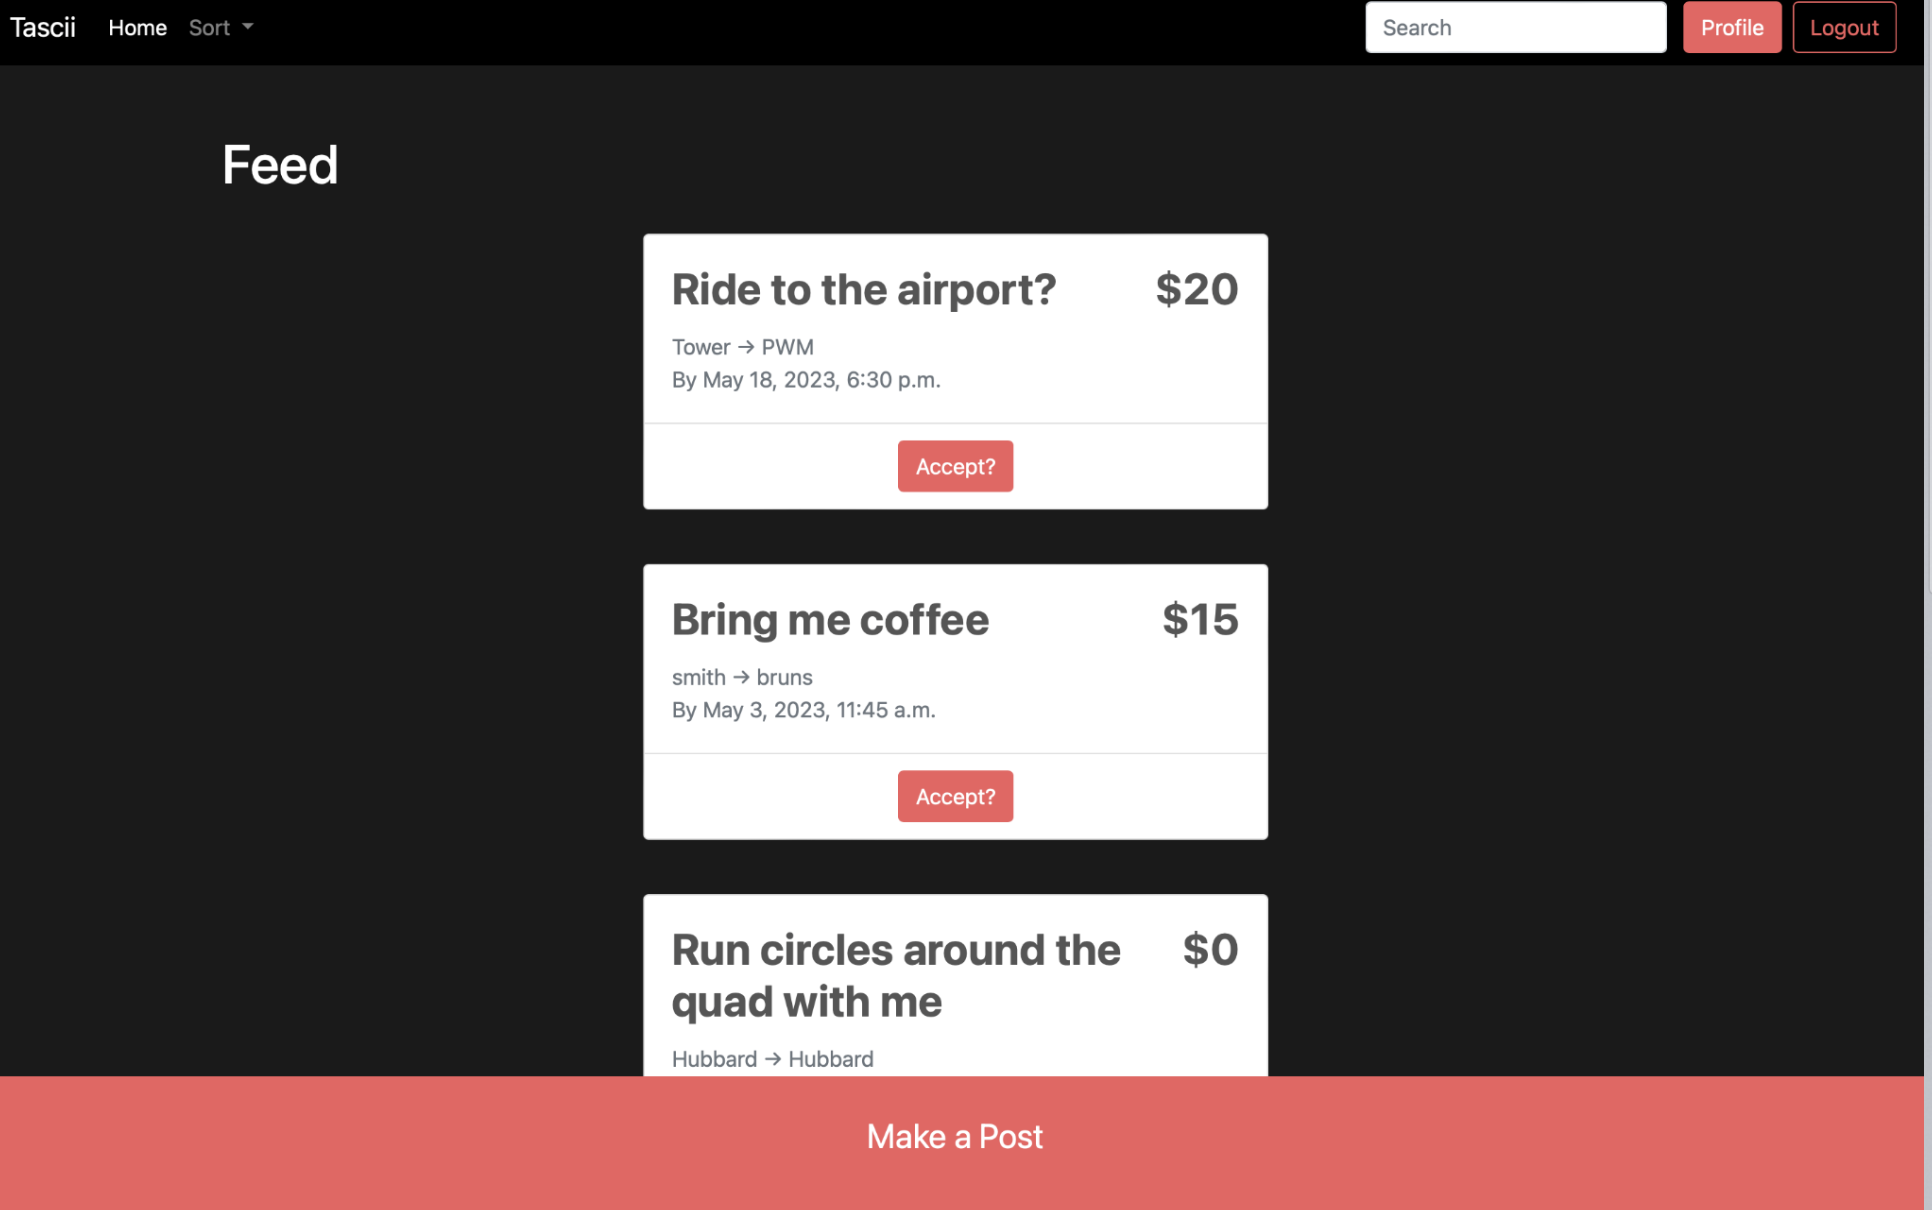
\includegraphics[width=1\textwidth]{images/Home.png}
        
        \label{fig:bird1}
    \end{figure}


We also wanted the feed to appear seamlessly for users that are both logged in and logged out. To do this we render the page dynamically based on whether the user has logged in and been authenticated. If users are not signed in, almost all of the buttons on the page direct them towards the login page (see fig. 6, 7). Similarly, the login and sign-up buttons become replaced with profile and logout buttons once the user is signed in.(see fig. 4, 5)

\begin{figure}
\centering
\begin{minipage}{.5\textwidth}
  \centering
  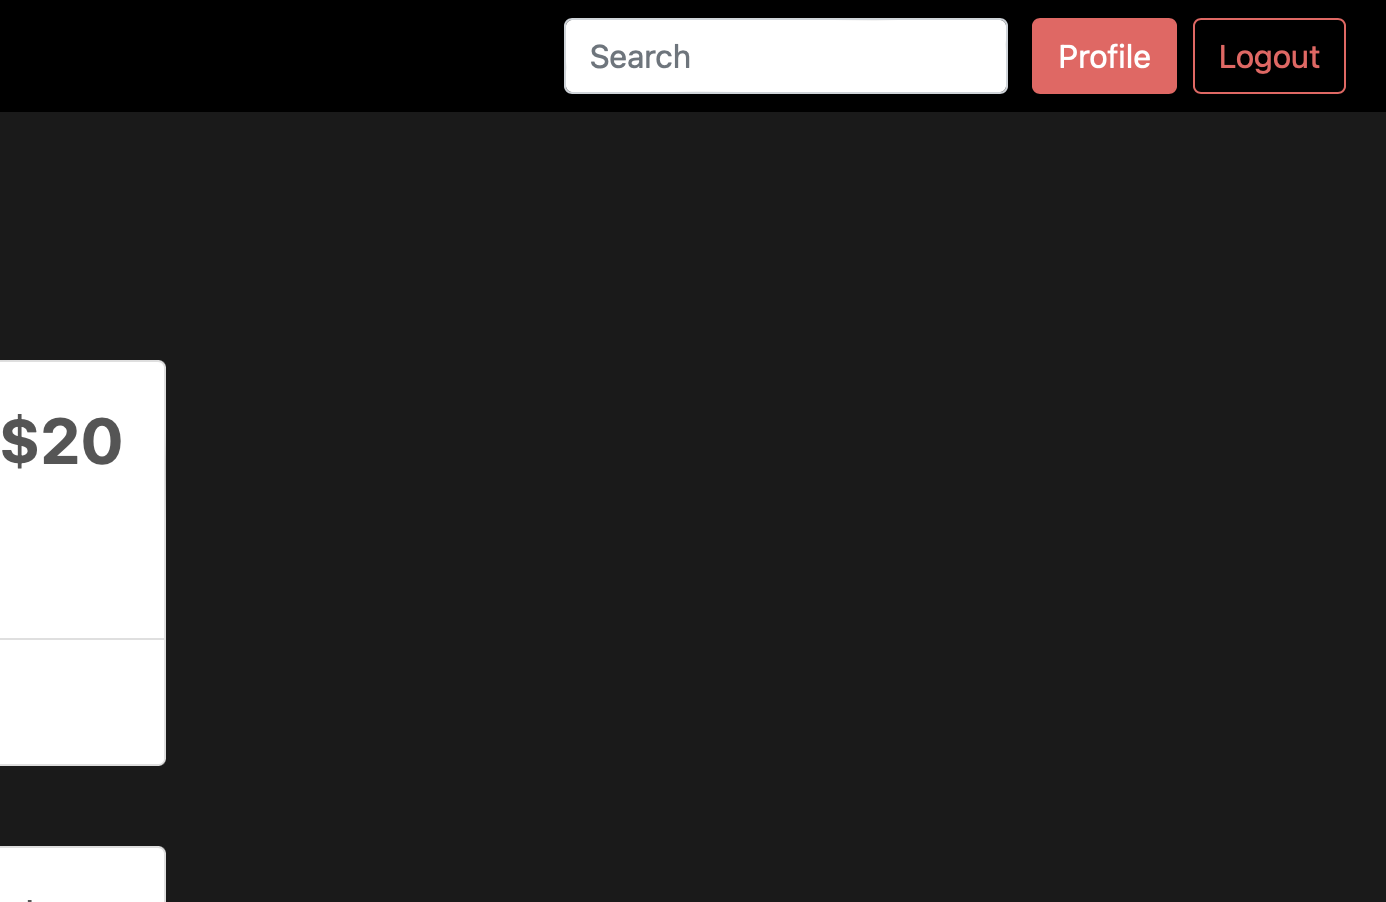
\includegraphics[width=.8\linewidth]{images/Loggedin.png}
  \captionof{figure}{Logged In}
  \label{fig:test1}
\end{minipage}%
\begin{minipage}{.5\textwidth}
  \centering
  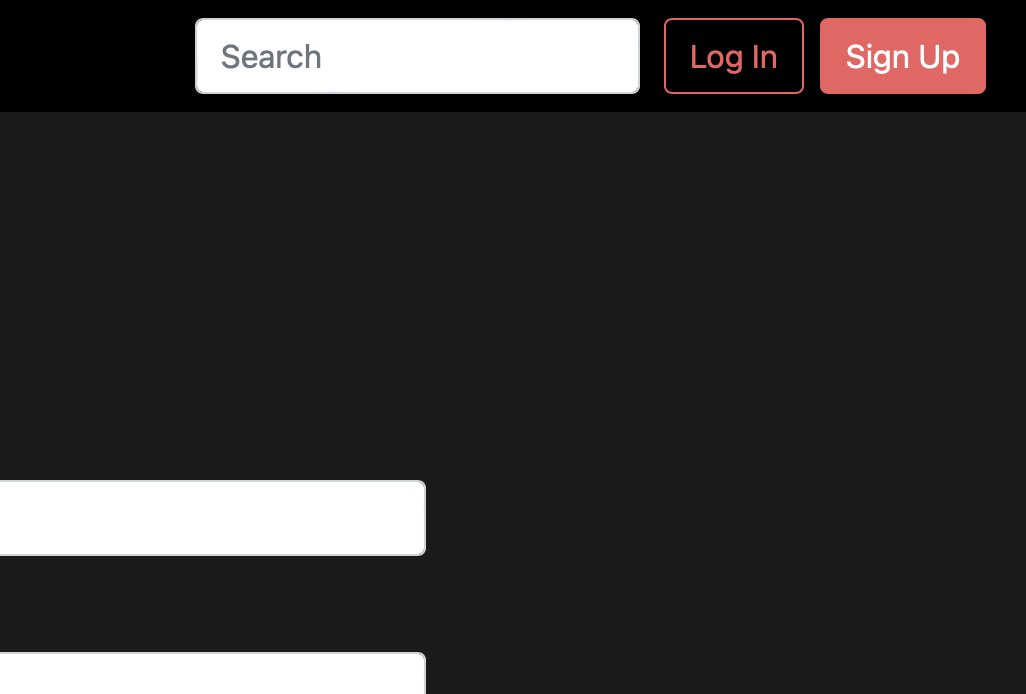
\includegraphics[width=.8\linewidth]{images/LoggedOut.png}
  \captionof{figure}{Logged Out}
  \label{fig:test2}
\end{minipage}
\end{figure}

\begin{figure}
\centering
\begin{minipage}{.5\textwidth}
  \centering
  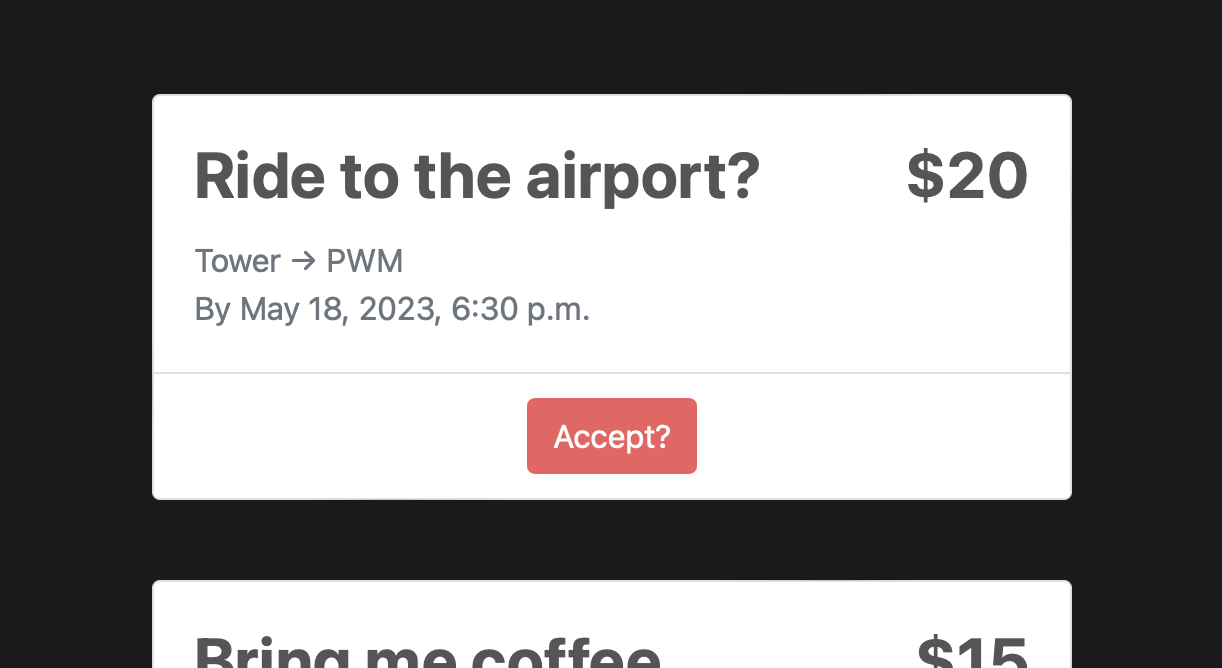
\includegraphics[width=.8\linewidth]{images/LoggedInPost.png}
  \captionof{figure}{Logged In}
  \label{fig:test1}
\end{minipage}%
\begin{minipage}{.5\textwidth}
  \centering
  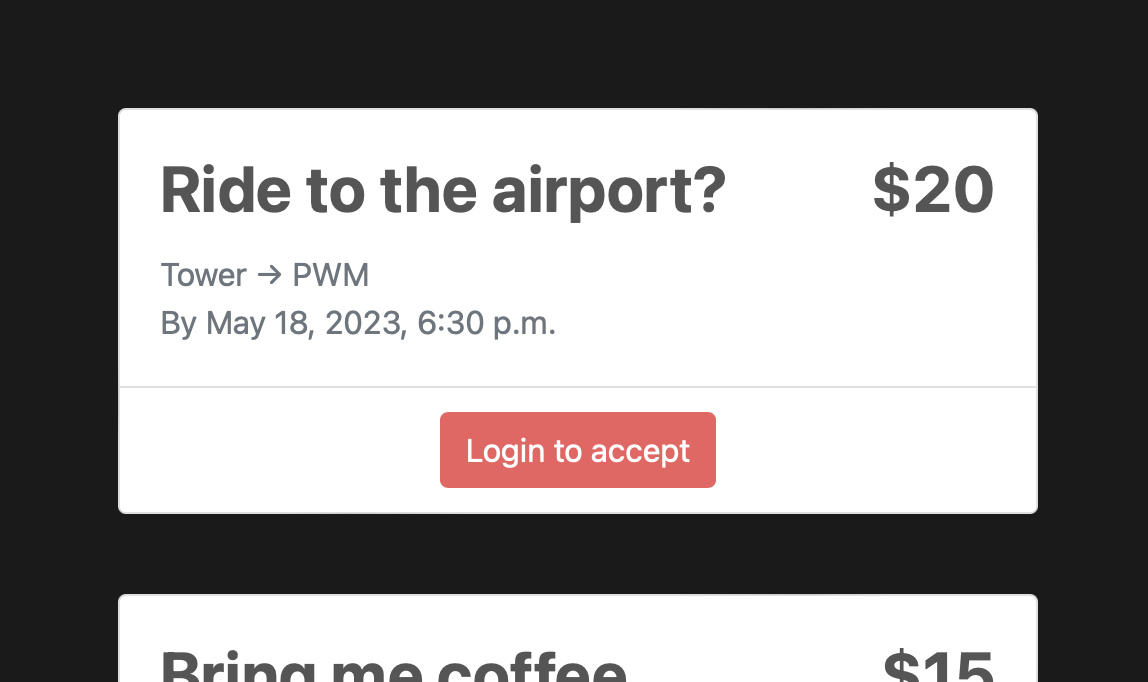
\includegraphics[width=.8\linewidth]{images/LoggedOutPost.png}
  \captionof{figure}{Logged Out}
  \label{fig:test2}
\end{minipage}
\end{figure}


Moreover, Tascii offers filtering and search options for the feed which enable users to narrow down their task search based on price, time, and recency (see fig.8). This functionality enhances efficiency by allowing users to focus on tasks that align with their preferences or are conveniently located. Our commitment to usability principles, specifically learnability and efficiency, led us to adopt a minimalist design throughout the app. This design approach not only minimizes confusion but also facilitates quick and seamless transactions, ensuring a user-friendly experience that meets the needs of college students.

\begin{figure}[ht]
        \centering
        \caption{filters}
        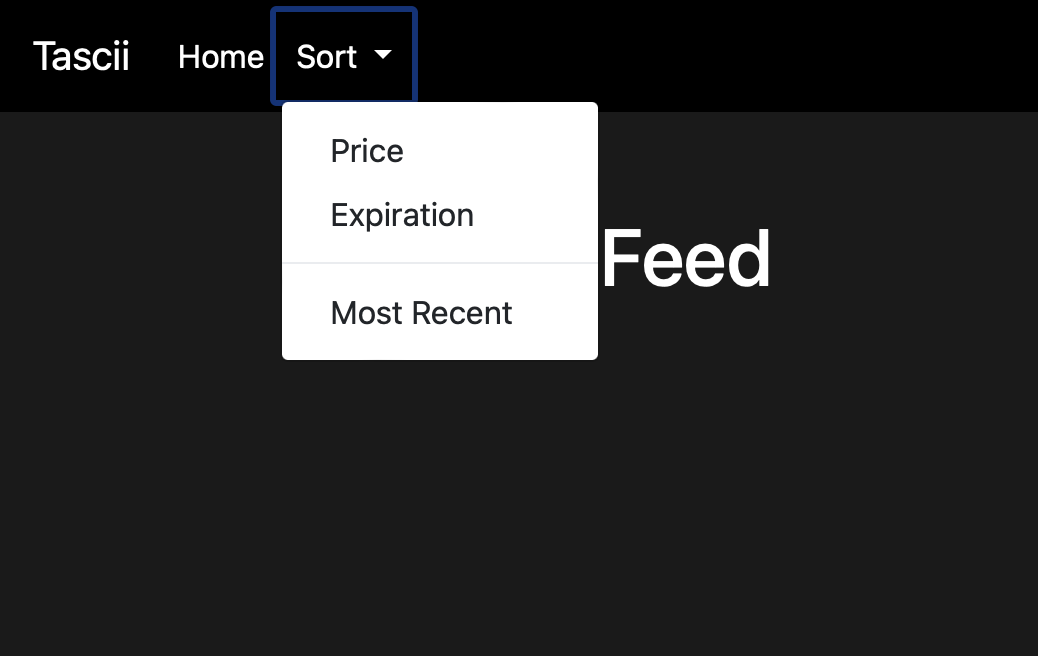
\includegraphics[width=1\textwidth]{images/Sort.png}
        
        \label{fig:bird1}
    \end{figure}

To use Tascii, users are required to create profiles and log in to the app, and these pages are both relatively simple and straightforward. By staying consistent with a layout that is common in other websites, the process is comfortable and familiar. The signup page provides interactive feedback if the input is invalid, and there are hints below some fields to guide users. The user's profile page serves as a hub for displaying essential information, such as their rating, completed tasks, and posted tasks. These statistics contribute to building trust among users and promoting high-quality interactions within the platform. It is also allows users to find critical information without having to remember it. Furthermore, we acknowledged the significance of accountability and reputation within the platform by incorporating a review system for deliveries and services. These design choices reflect our dedication to creating a professional and reliable platform that prioritizes user needs and experiences.

\begin{figure}[ht]
        \centering
        \caption{profile}
        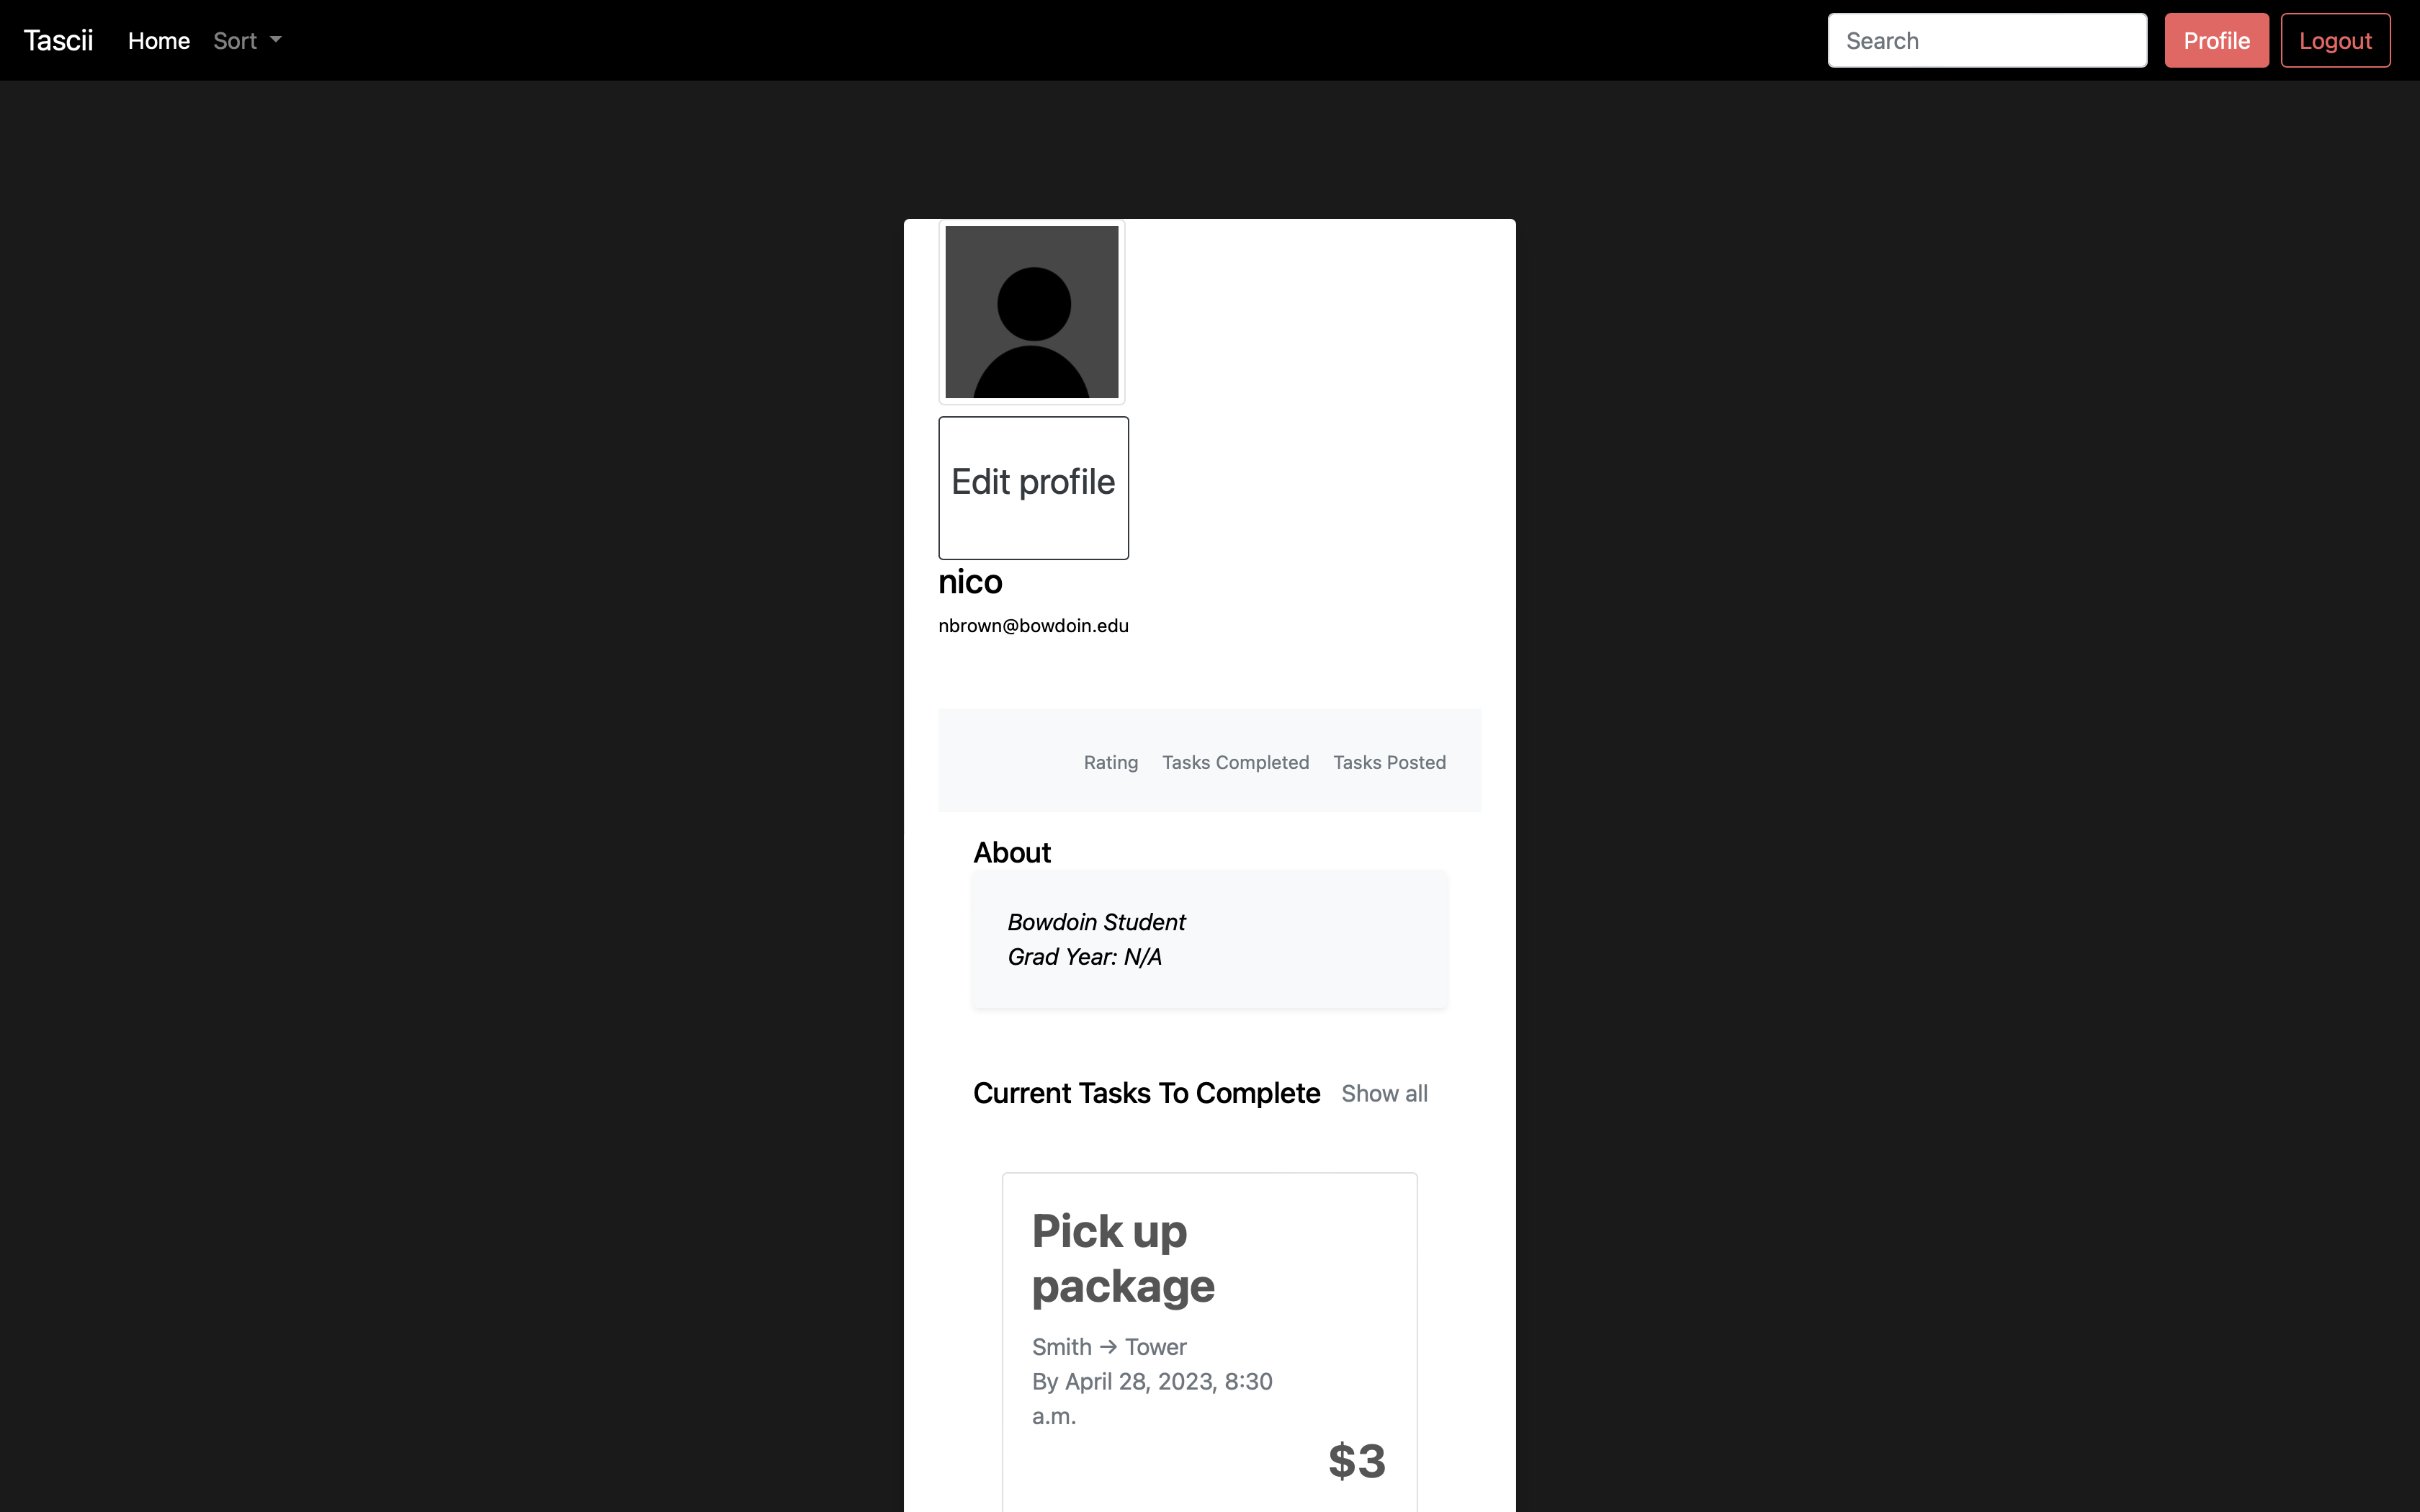
\includegraphics[width=1\textwidth]{images/Profile.png}
        
        \label{fig:bird1}
    \end{figure}

Users gave us feedback on our initial prototypes indicating that the design was a bit boring, so we added a scroll animation to make the experience a bit more engaging. We also chose to accent all of the prominent buttons with color to draw the users eye to the main actions available on the page. In a sense, we are using color as a signifier to highlight affordances within the design. Another fun feature is that for users using Arc browser, the accent color will match the theme of their browser window (video can be found on GitHub). 


\section{Methods}

To evaluate our high fidelity prototype, we designed an experiment to evaluate users’ perception of the design along with their efficiency when completing tasks. For this study, we used a convenience sample consisting of eight college students. These students were all in the same human computer interaction course, and they were mostly juniors and seniors. While this approach is often prone to sampling error, this sample is somewhat representative of our users given that college students are our target demographic. The small sample size is a notable limitation of the study, and working with computer science students may bias the results as the participants are likely more comfortable navigating the web. 

The experiment consisted of two tests that utilized a within-subjects design to compare our site with a competitor’s. For this study, we selected DoorDash since they are another online marketplace used to get help with delivery. To compare user efficiency across the two sites, we measured the time it took for users to sign in and place an order. We selected this task since it is the primary action users would take for both services, and they follow a similar workflow. The website and user interface were independent variables while the time to complete the task was the dependent variable. Across trials, users were shown the two sites in different orders to counterbalance and ensure that the order did not bias the study's results. To measure the aesthetic qualities of the two designs, we chose 18 words from the Microsoft Desirability Toolkit. These words were evenly distributed between adjectives with negative, neutral, and positive connotations. The order of the words were randomized, and users were asked to pick the three words that best described each design. We changed the order users would evaluate the sites in order to counterbalance. 

To conduct the study we used Apple’s 13-inch MacBook Pro which was released in 2022. Participants browsed the web using Safari for a browser, and random.org was used to generate a simple list of words in a random order. We also provided users with fake credit card information and the username and password for a premade DoorDash account.

While collecting the data, we worked with participants individually within a classroom setting. We used a script for interviewing users to ensure that the test was standardized for each participant. The full script is attached in the appendix. Users started the efficiency test from the home page of each website, and members from our team sat next to them to observe their progress and provide the login information for DoorDash. The sign-in process for DoorDash involves a text message verification, so we provided the code as soon as we received the text message for the premade account. We did not fully place the order to DoorDash, so we stopped timing once the participants had filled out the phony credit card information for the order. For the aesthetic measurements, we pulled up the list of adjectives and randomized the order before the participants selected three.


\section{Results}

Below are the times it took participants to sign in and make a post on the two websites. The average time to sign in and make a post on Tascii was one minute 29 seconds, while the average time on DoorDash was slightly longer at one minute 44 seconds. However, there was one notable outlier for DoorDash where the text message verification code took a long time to come through. When comparing the two samples, there is not statistically significant difference, and a paired sample t-test resulted in a p-value of 0.649. 

\begin{figure}[ht]
        \centering
        \caption{Description / time taken to post task on Taskii vs description / time taken to order food on DoorDash}
        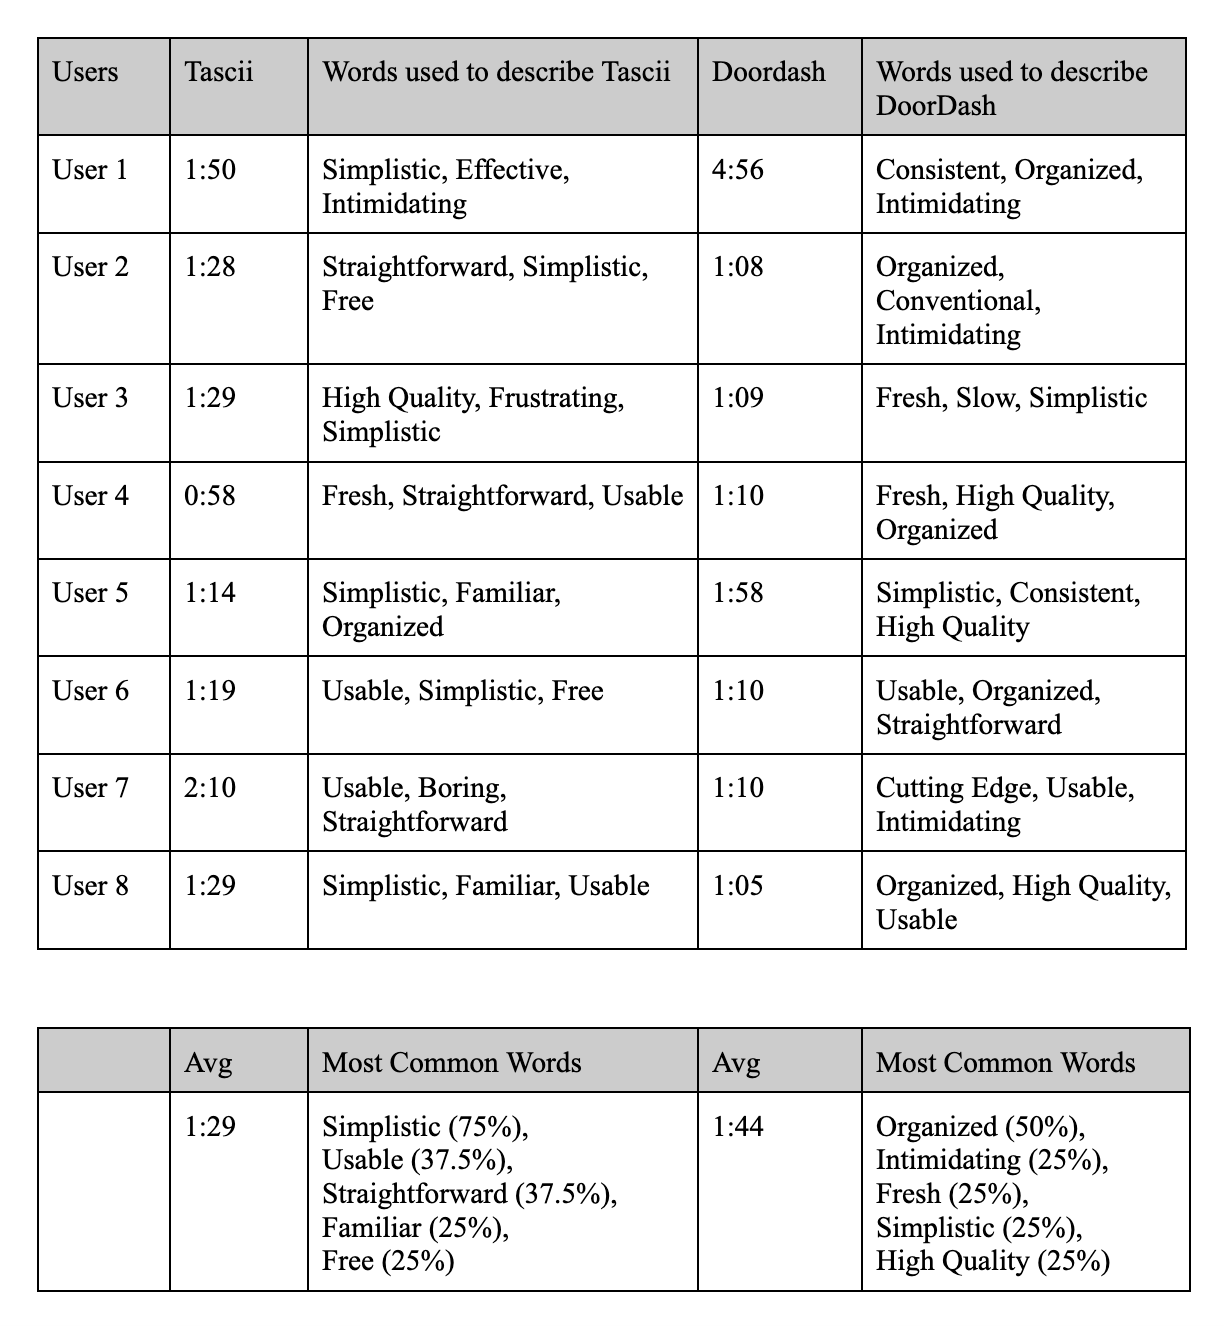
\includegraphics[width=1\textwidth]{images/Table.png}
        
        \label{fig:Data Table}
    \end{figure}


\section{Discussion}

The results from the study show that there is no significant difference in efficiency across the two designs. However, comparing the two processes highlighted some interesting differences. For example, DoorDash requires more rigorous authentication information to sign in as they have two step verification in place. While the design does not currently check if the user has a registered Bowdoin email, integrating with this alternative system has the potential to increase user efficiency. Additionally, we don't require any credit card information up front to make a post. Instead the platform leaves users to figure out their own payment method externally. Just like most casual interactions, users can text to follow up and choose whether they want to use cash, Venmo, or any other form of payment. 

The aesthetic descriptors also provided some interesting insights. 75\% of participants called our design simplistic while only 25\% described DoorDash that way. Instead, 25\% used the word intimidating where this never came up in our website. We believe this is because DoorDash's homepage displays a lot of filters, menus, and categories, so it comes across as overwhelming. DoorDash requires users to navigate through several menus in order to find a restaurant, while Tascii makes all posts available straight from the homepage. Our design displays posts sequentially, so only three or four are available at one time, and the navigation is direct and familiar. Once again, this is an advantage of serving a smaller community. Whereas DoorDash has to serve the entire country with thousands of restaurants, Tascii is able to present a more simplistic design with less market congestion. These descriptions may also be explained by the Hick-Hyman Law of Reaction Time which states that users take longer to react when confronted with more choices. 

However, despite the more rigorous login, added payment information, and increased number of options, DoorDash still had times that were comparable or faster than ours. We believe that this is because DoorDash is optimized for mobile devices where clicking and swiping are much faster than typing. Placing an order involved clicking through several menus, but there were almost no text fields. For first time users, inputting the credit card information took a while, but this information could be auto-completed for later orders. While our custom text fields make the interface more familiar and flexible, they have the downside of slowing users slightly.
	
Some limitations that prevent us from directly comparing similar services are inherent in the design of our product. Although some design elements are similar, the product as a whole is visually and technically different from other services. Another limitation is that DoorDash’s two factor authentication system proved to be inconsistent when sending out verification text messages. Although this is simply part of their system, the largest time differences are likely attributed to this step. Lastly, our limited sample size may limit the conclusions we are able to draw from this study.

Generally, our findings reinforced the topics and themes of Human Computer Interaction (HCI) that we studied throughout the semester. What was more telling was that even though we knew the basic design principles of HCI while making each iteration of our product there were always things that we overlooked. This further reinforced that the need finding, laddering techniques, and interviews at various stages of development are crucial to ensure you create a usable product. At each stage of development our team was confident that our product was usable and clean cut, but we continued to find areas that needed improvement from peer work and class discussion. For example, our team was quite happy with our first high fidelity mock up, yet through interviewing our peers we learned that to a new user there were many uncertainties. Lack of continuity throughout the application, unclear labeling, and a bland color scheme, are just a few issues that were uncovered in the early stages.

This research confirms the importance of interviewing users for feedback throughout the development process. It also shows that catering to your target users and context can help shape a solution that is valuable and unique. Our goal was to make an interface that was engaging and easy to use for Bowdoin students, and descriptors such as simplistic, usable, straightforward, and familiar help to affirm that we achieved this goal. Key components to this design were the simple navigation flow and flexible posts that allow users to adapt to a diverse array of use cases. Considering the context and needs of this specific community, we were able to create an effective and unique approach to an online marketplace.
    
     

\section{Appendix}

\subsection{Need-finding Survey Data}

\begin{figure}[ht]
        \centering
        \caption{Supply and Demand for Moving Cars}
        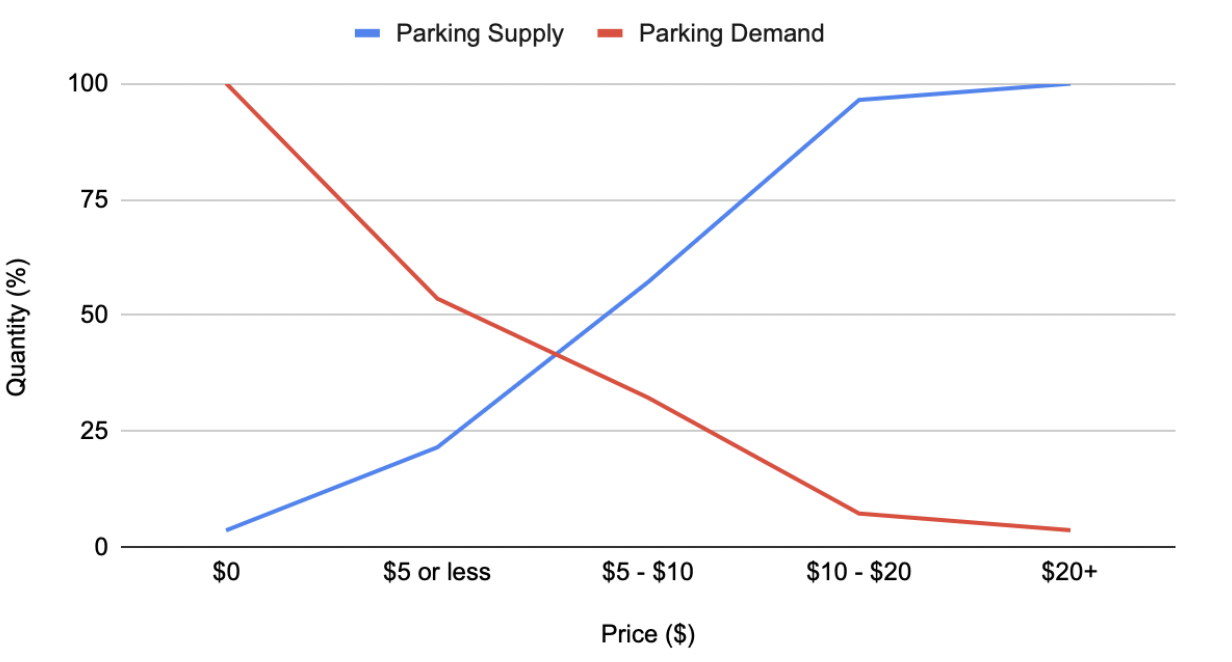
\includegraphics[width=1\textwidth]{images/cars.png}
        
        \label{fig:bird1}
    \end{figure}

\begin{figure}[ht]
        \centering
        \caption{Supply and Demand for Delivering Supers}
        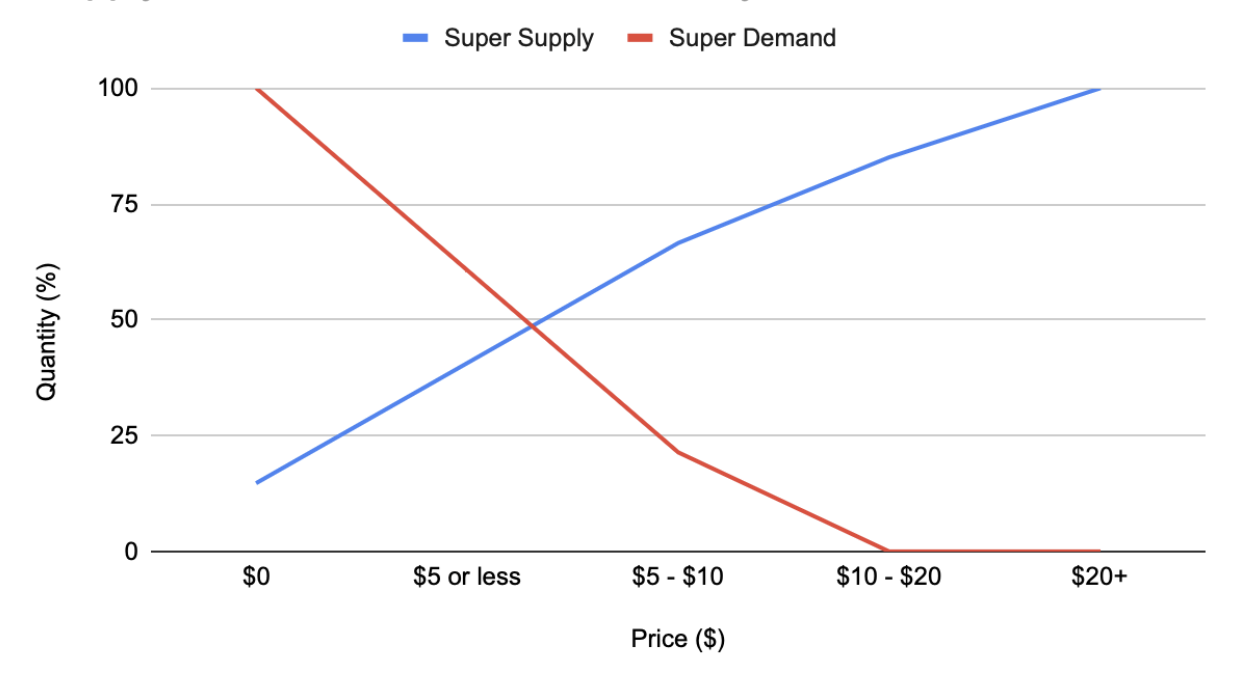
\includegraphics[width=1\textwidth]{images/supers.png}
        
        \;'[']]]1label{fig:bird1}
    \end{figure}


\begin{figure}[ht]
        \centering
        \caption{Most Wanted Service on Campus}
        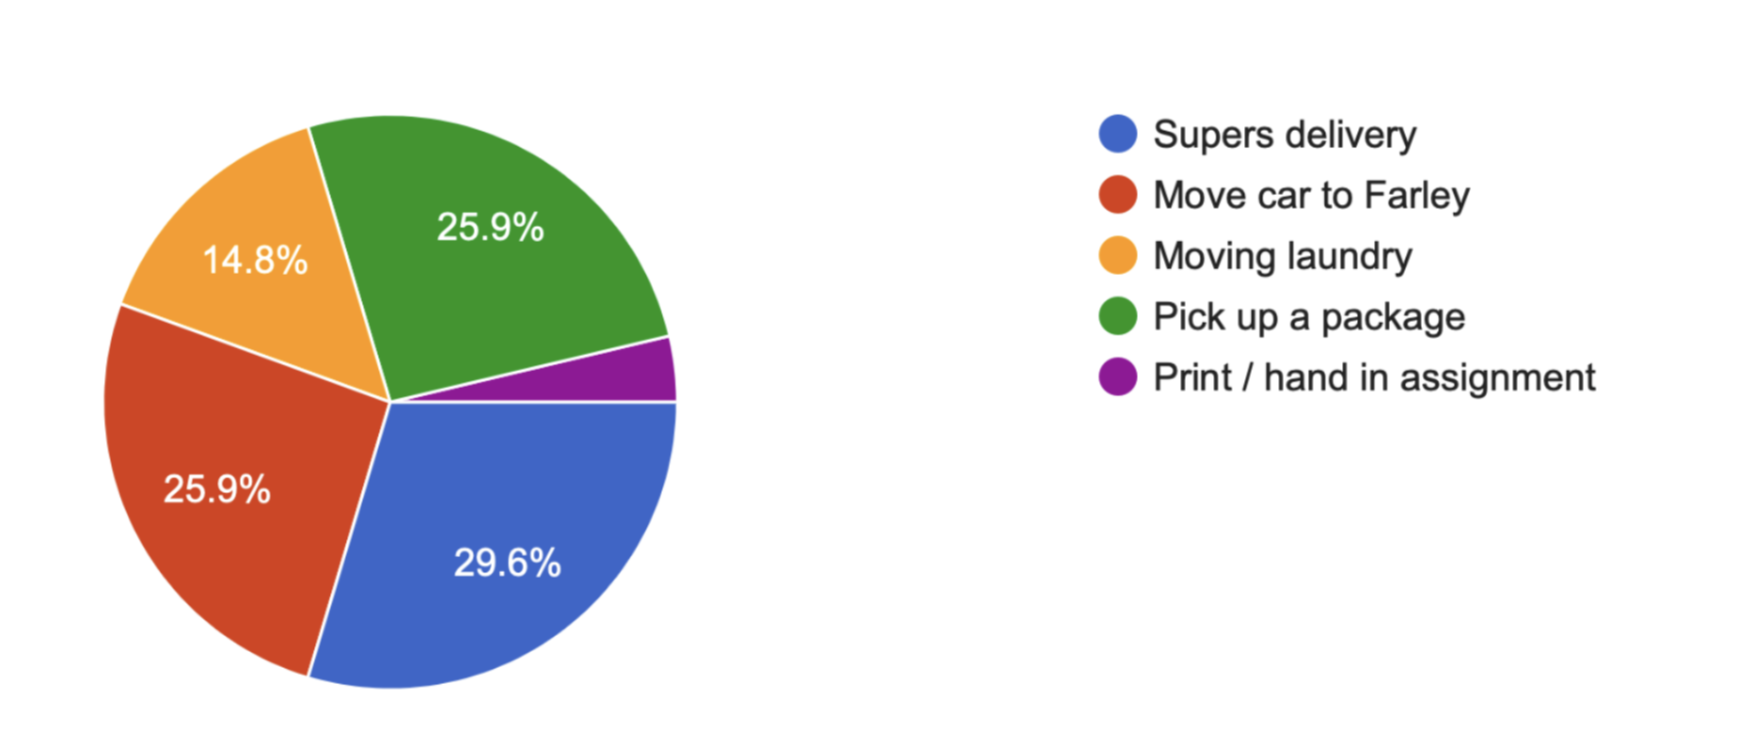
\includegraphics[width=1\textwidth]{images/pie.png}
        
        \label{fig:bird1}
    \end{figure}


\clearpage 
\subsection{Working Prototype Feedback}

After completing our initial interactive Figma prototype we had classmates test our product. We polled four students from the class and below are their major complaints and suggestions. \\

\begin{itemize}
\item Labels have a lack of naming clarity
\begin{itemize}
\item “My tasks” and “Active deliveries” have no continuity in what the actions are called.
\end{itemize}
\item Initial feature to “Counter” offer the poster of the task was unintuitive and many interviewees did not understand its purpose.
\item Lack of log showing your currently active tasks that you've posted, or the tasks that you've accepted to complete for others
\item Some users had difficulty navigating to the main feed after posting their task.
\item Difficult format to input expiration without calendar widget
\item No clear way to navigate back in the application and a user was stuck in a loop while trying to navigate out of the profile page.
\end{itemize}


\subsection{Script}

Hi I’m \_\_\_\_, 

We are making a platform for college students to post tasks they would want help with across campus. So, for example, if someone wants help moving their car to the student parking lot, they could make a post with the price they are willing to pay someone. For this study, we’re looking into how long it would take for someone to make a post like this. Later, we are also going to see what you think of the aesthetic of our design using some word associations.

First, I’m going to ask you to make a post on our site to see how long it takes. We’re also going to ask you to post an order on DoorDash because they’re a comparable company to us.

Do you have any questions about the task?

(Have participant complete the task)

Tell the user to log in 

Tell the user to make a post 

Ok great! Next I am going to show you a series of words that could describe our current design, and I’ll ask you to pick the top three words that you think are the most applicable. Do you have any questions?

Thanks for your time, and if you have any other questions you can email me at asdf@bowdoin.edu


\section{Acknowledgments}

We would like to take this opportunity to express our sincere gratitude to all the participants who took part in our usability studies and the anonymous Bowdoin students who responded to our needfinding survey. Without their valuable contribution, this research would not have been possible. We would also like to extend our thanks to Django, an incredibly helpful framework and resource, which facilitated the development of our web application. We are grateful to Professor Harmon for her guidance and feedback throughout the course of this project. Finally, we thank Bowdoin College for providing us with the resources and support necessary to carry out this research.

\clearpage
\section{Bibliography}

\bibitem{Cooper}
Cooper, James M., Megan E. Lee, and Brishen Rogers. "The 

Economic Impacts of Ridesharing: Driver

Earnings and Employment in the Rideshare Industry." 

Working Paper Series, no. 2016-14 (2016):

1-41. {https://openresearch-

repository.anu.edu.au/bitstream/1885/216366/1/8180%20Uber.

pdf}.\\

\bibitem{Elder-Vass}
Elder-Vass, Dave. "Commerce, Community and Digital 

Gifts." In \textit{The Social Life of Money}, edited by

Nigel Dodd, 214-229. New York: Routledge, 2017.

https://www.taylorfrancis.com/chapters/edit/10.4324/9

781315737171-15.\\

\bibitem{Kalleberg}
Kalleberg, Arne L., and Michael Dunn. “Good Jobs, Bad 

Jobs in the Gig Economy.” \textit{Perspectives on

Work} 20 (2016): 10–75. 

http://www.jstor.org/stable/26621129.\\

\bibitem{Learning}
"Learning to Airbnb by Engaging in Online Communities of 

Practice."

https://dl.acm.org/doi/pdf/10.1145/3359330.\\

\bibitem{Market}
"Market Design for HCI: Successes and Failures of Peer-to-

Peer Exchange Platforms."

https://dl.acm.org/doi/pdf/10.1145/3025453.3025515.\\

\bibitem{Park}
Park, Haewoon. "Towards an Understanding of the Effects 

of Social Media on Political Participation."
\textit{ACM CCS '16: Proceedings of the 2016 ACM 

Conference on Computer and Communications

Security}, ACM, New York, NY, USA, 2016, pp. 1065-1080.\\

\bibitem{Roose}
Roose, Kevin. "Facebook is Weaker Than We Knew." 

\textit{The New York Times}, 4 Oct. 2021,

https://www.nytimes.com/2021/10/04/technology/faceboo

k-files.html.\\

\bibitem{Seyfang}
Seyfang, G. (2003), Growing cohesive communities one 

favour at a time: social exclusion, active

citizenship and time banks. \textit{International Journal 

of Urban and Regional Research}, 27: 699-706.

https://doi.org/10.1111/1468-2427.00475.\\

\bibitem{Smith}
Smith, J. Walker. “The Uber-All Economy of the Future.” 

\textit{The Independent Review} 20, no. 3 (2016):

383–90. http://www.jstor.org/stable/24562159.\\

\bibitem{Reciprocity}
"Why do you return the favor in online knowledge 

communities? A study of the motivations of reciprocity."

https://www.sciencedirect.com/science/article/pii/S07

47563216303314.\\

\bibitem{Uber}
Uber. "Safety."

https://www.uber.com/us/en/ride/safety/?

uclick\_id=58abd988-91d0-4969-97d0-423a3dd436d2.


